%\documentclass[10pt]{beamer}
%\documentclass[10pt,aspectratio=169]{beamer}
\documentclass[handout,10pt,aspectratio=169]{beamer}
%\includeonlyframes{current}
\usepackage{textcomp,colortbl}
\usepackage{amsmath, amssymb, etoolbox, bm, listings}
\usepackage{animate, multirow, hyperref, color, longtable}
\usepackage{makeidx, multicol}
\usepackage[retainorgcmds]{IEEEtrantools}
\hypersetup{
  pdftitle={Designing ront Ends},
  colorlinks=true,
  citecolor={blue},
  urlcolor={blue},
  pdfcreator={LaTeX via pandoc}}

% These commands are from stack exchange. They are for creating the index of
% examples.
\makeindex
\newenvironment{theindex}
 {\let\item\par
  %definitions for subitem etc
  }{}
\newcommand\indexspace{}

\newcommand{\topic}{04}
\newcommand{\bb}{\mathbb}
\newcommand{\rlang}{\texttt{R} }
\newcommand{\ud}{\,\mathrm{d}}

%\includeonlyframes{current}
\setbeamertemplate{theorems}[numbered]
%\setbeameroption{show notes}
\undef{\example}
\theoremstyle{example}
\newtheorem{example}{\translate{Example}}

\DeclareMathOperator{\var}{var}
\DeclareMathOperator{\cov}{cov}
\DeclareMathOperator{\cor}{cor}
%\DeclareMathOperator{\dp}{dp}
\DeclareMathOperator{\ds}{ds}
\DeclareMathOperator{\dt}{dt}
\DeclareMathOperator{\du}{du}
\DeclareMathOperator{\dv}{dv}
\DeclareMathOperator{\dw}{dw}
\DeclareMathOperator{\dx}{dx}
\DeclareMathOperator{\dA}{dA}
\DeclareMathOperator{\dy}{dy}
\DeclareMathOperator{\dz}{dz}
\DeclareMathOperator{\dr}{dr}
\DeclareMathOperator{\dtheta}{d\theta}
\DeclareMathOperator{\SD}{SD}
\DeclareMathOperator{\Be}{Be}
\DeclareMathOperator{\Bin}{Bin}
\DeclareMathOperator{\Geom}{Geom}
\DeclareMathOperator{\Poi}{Poisson}
\DeclareMathOperator{\Exp}{Exp}

\DeclareMathOperator{\di}{d}
\newcommand{\ddx}{\frac{\di}{\dx}}
\newcommand{\ddz}{\frac{\di}{\dz}}
\newcommand{\ddxt}{\tfrac{\di}{\dx}}
\newcommand{\dydx}{\frac{\dy}{\dx}}
\newcommand{\dydxt}{\tfrac{\dy}{\dx}}
\newcommand{\pdx}[1]{\frac{\partial {#1}}{\partial x}}
\newcommand{\pdy}[1]{\frac{\partial {#1}}{\partial y}}
\newcommand{\rll}[1]{\texttt{#1}}

\usetheme{Boadilla}
\usecolortheme{dove}
%\usetheme[hideallsubsections]{PaloAlto}
% Control the style of bullets:
\setbeamertemplate{enumerate items}[circle]
\setbeamertemplate{section in toc}[circle]
\setbeamercolor{block title}{bg=cyan}
%setbeamercolor{block title}{bg=yellow}
\renewcommand<>\cellcolor[1]{\only#2{\beameroriginal\cellcolor{#1}}}

\setbeamertemplate{footline}[text line]{%
  \parbox{\linewidth}{\vspace*{-8pt}\insertshorttitle\hfill\insertshortauthor\hfill\insertpagenumber}
}
\setbeamertemplate{navigation symbols}{}

\title[]{ Designing Front-Ends }
\author[Topic \topic]{Vik Gopal}
\date{DSA3101 AY 22/23 Sem II}

\begin{document}
\lstset{
  upquote=true,
  basicstyle=\ttfamily,
  backgroundcolor=\color{yellow!10},
  showstringspaces=false}
\maketitle
\section*{Outline}
\frame{\tableofcontents}

\section{Shiny}
\subsection{Introduction to Shiny}

\begin{frame}{What is Shiny?}
\begin{columns}[t]
\begin{column}{8cm}
\begin{itemize}
\item
  Shiny is an R package for making interactive web applications.
\item
  Web applications can be:
  \begin{itemize}
  \item
    a front-end for interacting with a model API.
  \item
    for interacting with the results of an analysis.
  \item
    for exploring a dataset or a model.
  \end{itemize}
\item
  Shiny web applications need to be hosted on a Shiny server.
  \begin{itemize}
  \item
    Docker containers are available
  \end{itemize}
\end{itemize}
\end{column}
\begin{column}{6cm}
\begin{center}
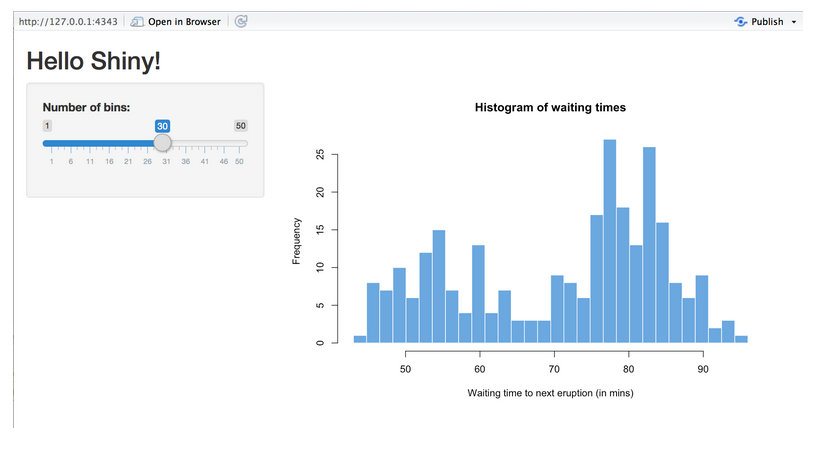
\includegraphics[width=0.9\linewidth]{figs/shiny-hello-01} 
\end{center}
\end{column}
\end{columns}
\end{frame}

\begin{frame}{A first Shiny application}
\begin{columns}[t]
\begin{column}{8cm}
\begin{enumerate}
\def\labelenumi{\arabic{enumi}.}
\item
  Shiny applications are contained in a folder of their own. There must
  be a file called \texttt{app.R} in this folder.
\item
  This file contains the definition of the two fundamental parts of
  every Shiny application: \texttt{ui} and \texttt{server}
\end{enumerate}
\end{column}
\begin{column}{6cm}
\begin{center}
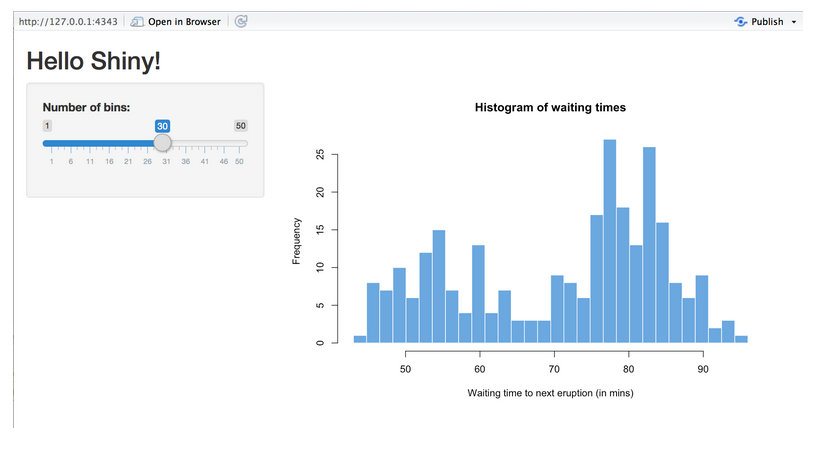
\includegraphics[width=0.9\linewidth]{figs/shiny-hello-01} 
\end{center}
\end{column}
\end{columns}
\end{frame}

\begin{frame}{Shiny ui definition}
\begin{columns}[t]
\begin{column}{7cm}
    \begin{center}
    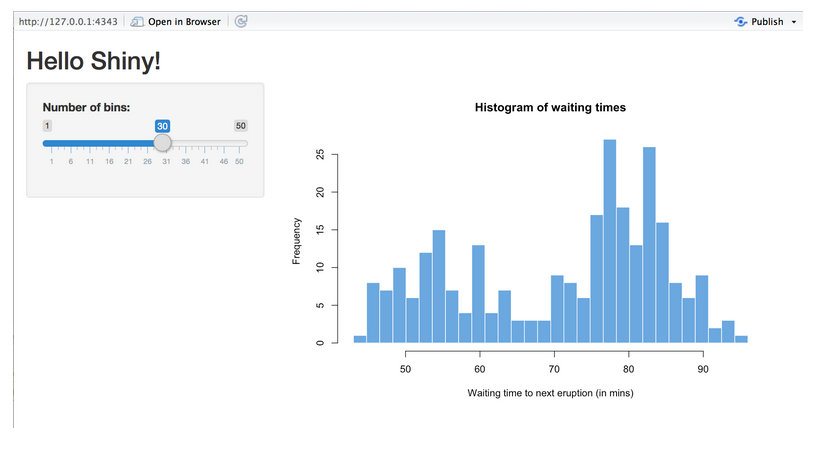
\includegraphics[width=0.95\linewidth]{figs/shiny-hello-01} 
    \end{center}
\end{column}
\begin{column}{7cm}
    \begin{center}
    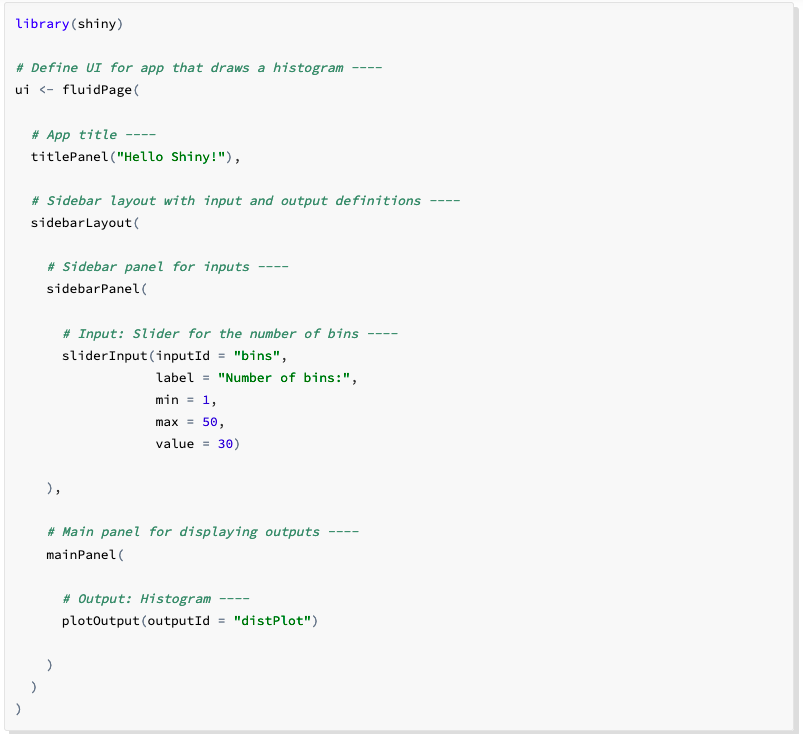
\includegraphics[width=1.0\linewidth]{figs/shiny-hello-ui} 
    \end{center}
\end{column}
\end{columns}
\end{frame}

\begin{frame}{Shiny server definition}
\begin{columns}[t]
\begin{column}{7cm}
    \begin{center}
    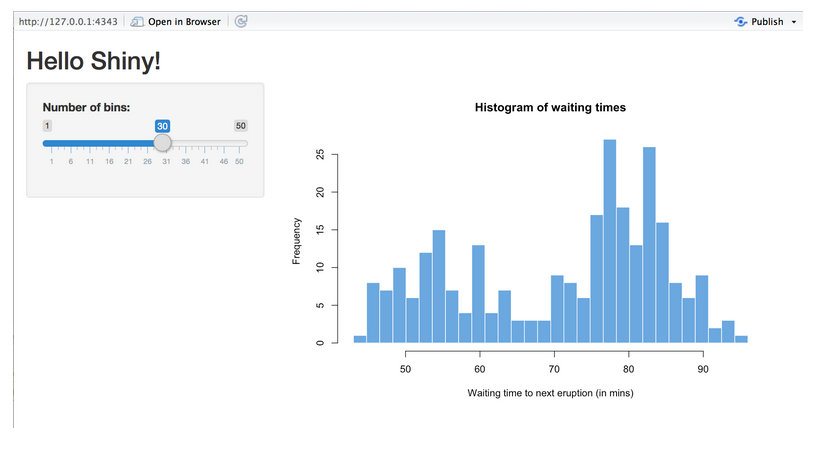
\includegraphics[width=0.95\linewidth]{figs/shiny-hello-01} 
    \end{center}
\end{column}
\begin{column}{7cm}
    \begin{center} 
    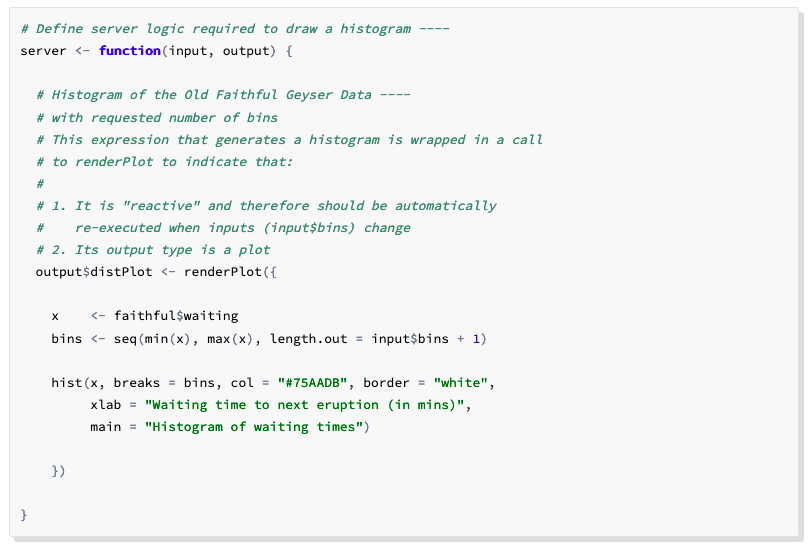
\includegraphics[width=1.0\linewidth]{figs/shiny-hello-server}
    \end{center}
\end{column}
\end{columns}
\end{frame}

\begin{frame}{Summary}
\begin{itemize}
\item
  \texttt{ui} is an R object that defines
  \begin{itemize}
  \item
    the input elements that the user interacts with
  \item
    the output elements that the application will render
  \item
    the layout of these two elements
  \item
    input and output elements have an id
  \end{itemize}
\item
  \texttt{server} is an R function that defines the logic of the
  application:

  \begin{itemize}
  \item
    e.g.~what to do when a particular input element is changed.
    \begin{itemize}
    \item
      For each
    \end{itemize}
  \item
    the server automatically detects and reacts to changes in input
    elements.
  \item
    input elements are referenced here using \texttt{input\$\_\_\_}
    notation within \textbf{reactive} code sections.
  \item
    output elements are referenced using \texttt{output\$\_\_\_}
    notation.
  \end{itemize}
\end{itemize}
\end{frame}

\subsection{Shiny Layouts}
\frame{\tableofcontents[currentsubsection]}

\begin{frame}{Layout of the UI}
\begin{itemize}
\item The UI is essentially a HTML page, with custom styling.
\item Later on, we shall see how we can use HTML/CSS to improve the look of our
UI, but the bulk of our work can be done through R.
\item There are a few typical layouts that we should know about. We can then
combine them and/or nest them to achieve more complicated layouts.
\end{itemize}
\end{frame}

\begin{frame}{Sidebar layout}
\begin{center}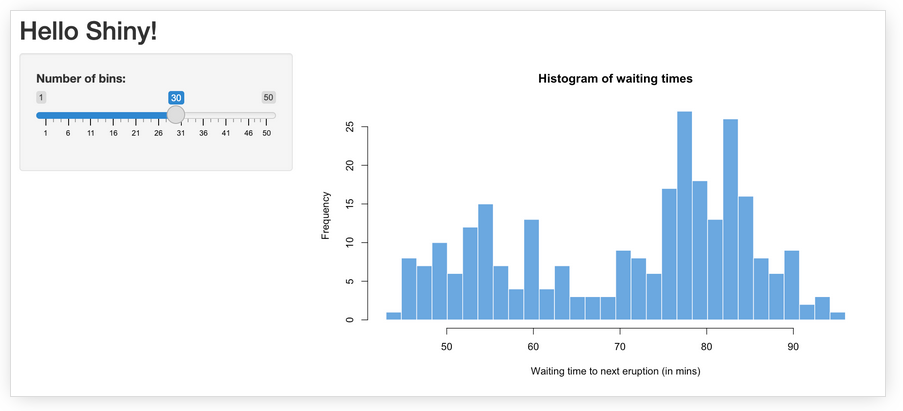
\includegraphics[width=0.9\linewidth]{figs/shiny-sidebar-layout} \end{center}
\end{frame}

\begin{frame}{Grid layout}
\begin{center}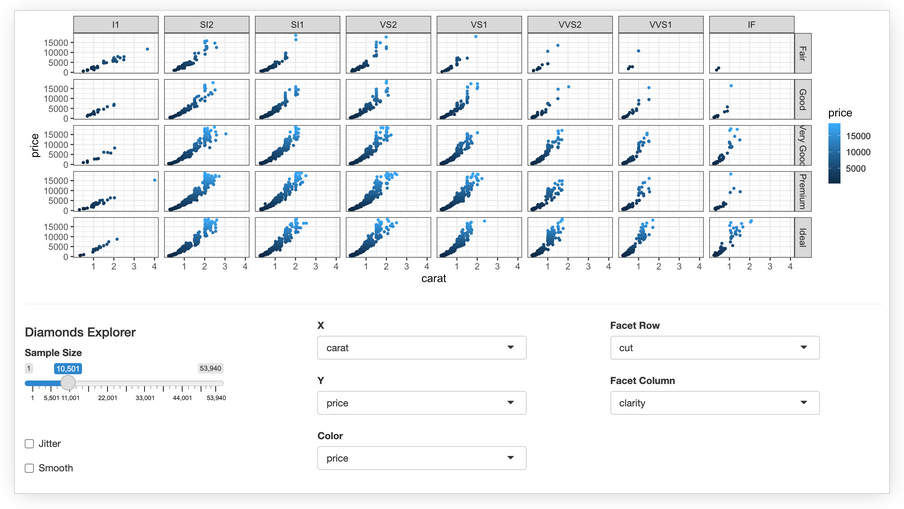
\includegraphics[width=0.9\linewidth]{figs/shiny-grid-layout} \end{center}
\end{frame}

\begin{frame}{Tabset layout}
\begin{center}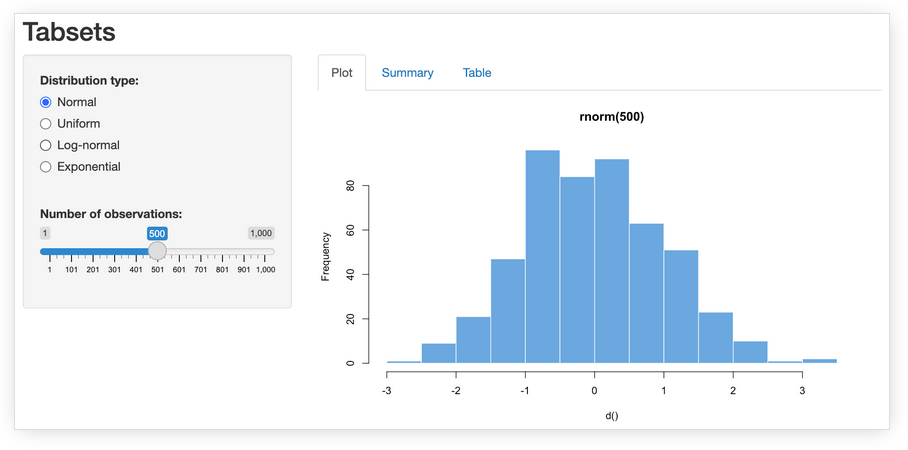
\includegraphics[width=0.9\linewidth]{figs/shiny-tabset-layout} \end{center}
\end{frame}

\begin{frame}{Navbar layout}
\begin{center}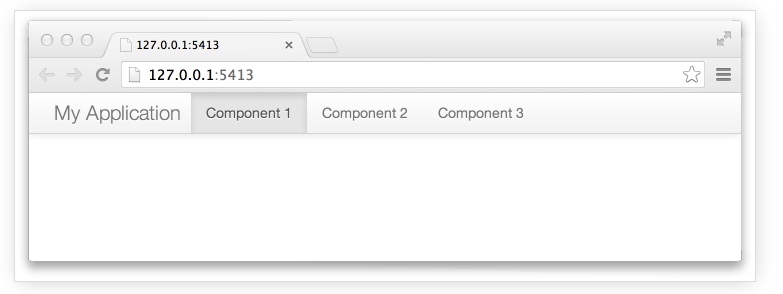
\includegraphics[width=0.6\linewidth]{figs/shiny-navbar-layout} \end{center}
\begin{center}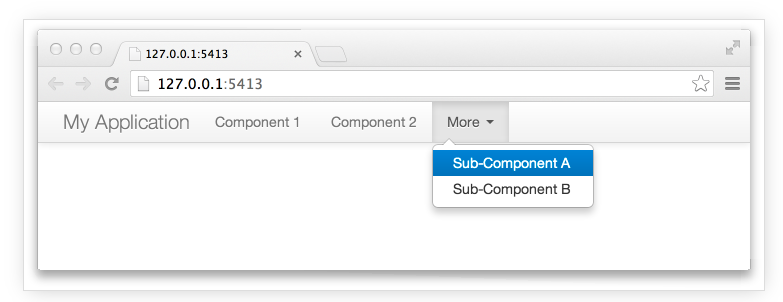
\includegraphics[width=0.6\linewidth]{figs/shiny-navbar-layout2} \end{center}
\end{frame}

\begin{frame}[fragile]{Defining Columns}
\begin{columns}[t]
\begin{column}{5cm}

\begin{center}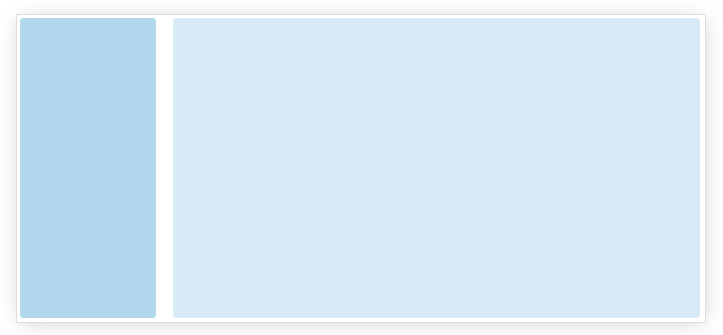
\includegraphics[width=1.0\linewidth]{figs/shiny-define-cols} 
\end{center}

\end{column}
\begin{column}{9cm}
\begin{lstlisting}
ui <- fluidPage(
  fluidRow(
    column(2,
      "sidebar"
    ),
    column(10,
      "main"
    )
  )
)
\end{lstlisting}
\end{column}
\end{columns}
\end{frame}

\begin{frame}[fragile,shrink=15]{Defining Nested Columns}
\begin{columns}[t]
\begin{column}{8cm}

\begin{center}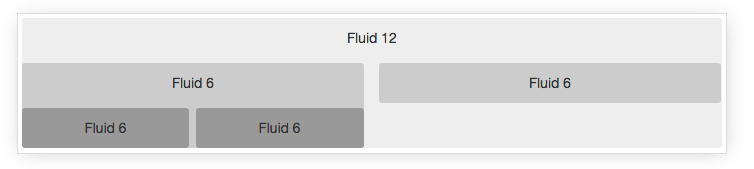
\includegraphics[width=0.9\linewidth]{figs/shiny-nested-cols}
\end{center}

\end{column}
\begin{column}{7cm}
\begin{lstlisting}
ui <- fluidPage(
  fluidRow(
    column(12,
      "Fluid 12",
      fluidRow(
        column(6,
          "Fluid 6",
          fluidRow(
            column(6, 
              "Fluid 6"),
            column(6,
              "Fluid 6")
          )
        ),
        column(width = 6,
          "Fluid 6")
      )
    )
  )
)
\end{lstlisting}
\end{column}
\end{columns}
\end{frame}


\begin{frame}{Control Widgets}
\begin{center}
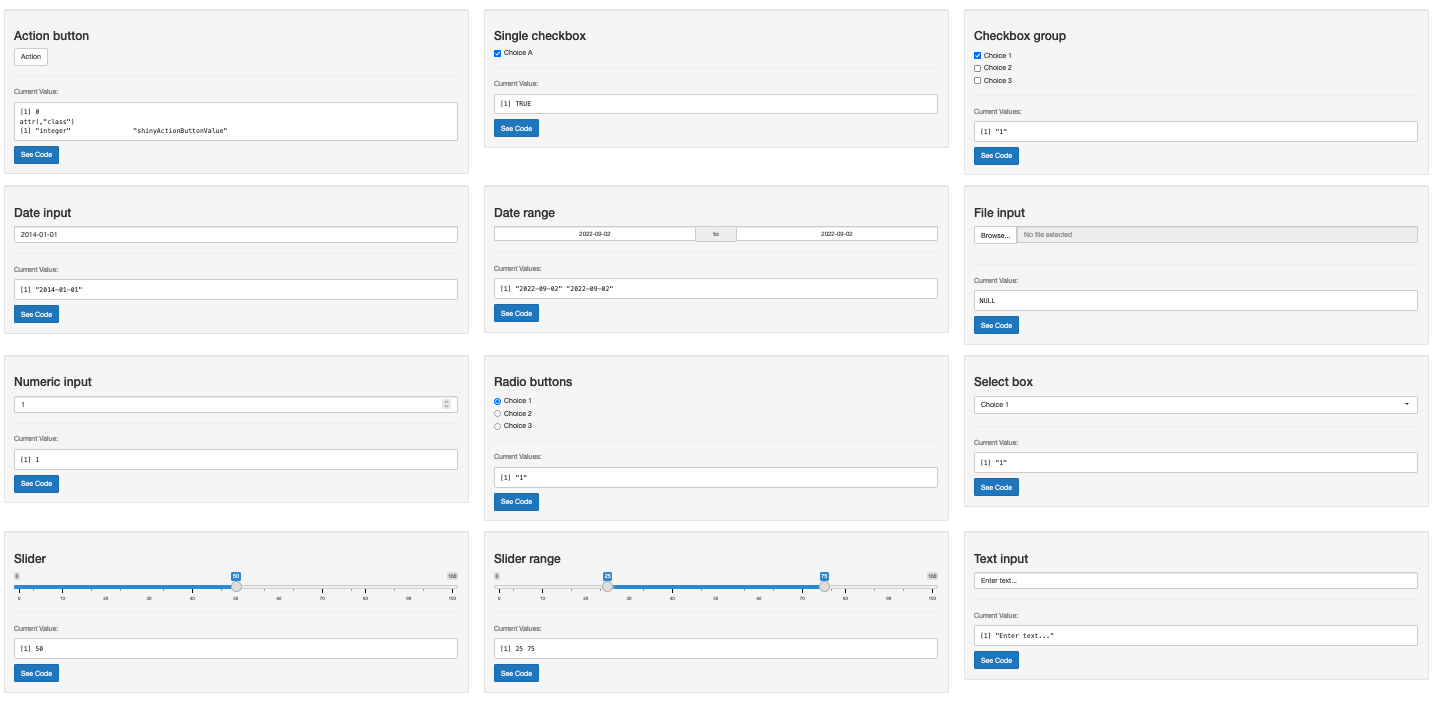
\includegraphics[width=0.9\linewidth]{figs/shiny-widgets} 
\end{center}
\end{frame}

\subsection{Reactivity}
\frame{\tableofcontents[currentsubsection]}

\begin{frame}{Reactivity}
\begin{itemize}
\item Reactivity is what allows Shiny to update output elements automatically.
\item It is both a bane and a boon for us.
\end{itemize}

\begin{center}
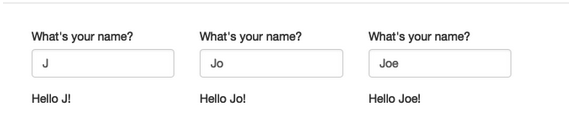
\includegraphics[width=0.8\linewidth]{figs/shiny-reactivity} 
\end{center}
\end{frame}

\subsection{Shiny Server}
\frame{\tableofcontents[currentsubsection]}

\begin{frame}[fragile]{Shiny Server}
\begin{itemize}
\item Until now, we have been running Shiny applications on our local machine.
\item When we want a user to access our front-end, we need to host it somewhere. This means we need to run a 
server, that can host all our Shiny applications.
\item To do so, we can use docker:
\begin{lstlisting}
docker run --name shiny-01 -d -p3838:3838 rocker/shiny
\end{lstlisting}
\item The above runs a Shiny server at port 3838. It already contains the 12 default Shiny examples that we have seen 
in this workshop. The following URLs should now work on your computer.
\begin{enumerate}
\item \url{http://localhost:3838}
\item \url{http://localhost:3838/01_hello}
\item \url{http://localhost:3838/03_reactivity}
\end{enumerate}
\end{itemize}
\end{frame}


\begin{frame}{Getting the Shiny Server Container to Host \emph{Your} Application}

\begin{enumerate}
\item Make sure the application works on your local machine.
\item Make a note of the libraries that it needs in order to run.
\item Include instructions in the Dockerfile to install these packages in the image.
\item Copy your application folder to \texttt{/src/shiny-server/} within the image.
\item When you run the container, your application should appear at 
\url{http://localhost:3838/<app-name>}.
\item If there are errors, open a terminal \textbf{in the container}, 
and navigate to \texttt{/var/logs/shiny-server/} to view the log files.
\end{enumerate}
\end{frame}


\subsection{References}
\begin{frame}{Shiny references}
\begin{enumerate}
\def\labelenumi{\arabic{enumi}.}
\item
  \href{https://shiny.rstudio.com/tutorial/written-tutorial/lesson1/}{Getting
  started with Shiny}
\item
  \href{https://mastering-shiny.org/}{Mastering Shiny}
\item
  \href{https://shiny.rstudio.com/articles/layout-guide.html}{Shiny
  Application Layout Guide}
\item
  \href{https://shiny.rstudio.com/articles/cheatsheet.html}{Shiny cheat
  sheet}
\item
  \href{https://datacamp.com}{Building Web Applications with Shiny in R
  DataCamp Course}
\item Customising the look and feel of your Shiny application using the 
\href{https://rstudio.github.io/bslib/index.html}{bslib R package}.
\end{enumerate}
\end{frame}


\section{HTML and CSS}
\subsection{HTML Basics}\label{html-basics}
\frame{\tableofcontents[currentsubsection]}

\begin{frame}{HyperText Markup Language}
\begin{itemize}
\item
  HTML consists of a series of elements, which \emph{mark up} different
  parts of content to make it appear a certain way.
\item
  Elements are defined by tags that enclose content.
\end{itemize}
\begin{center}
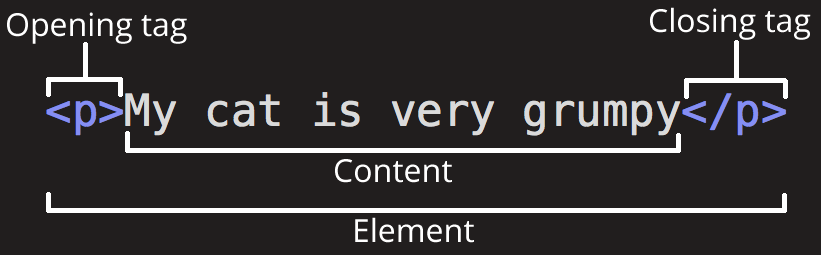
\includegraphics[width=0.7\linewidth]{figs/grumpy-cat-small-anatomy-html-element} 
\end{center}

\begin{itemize}
\item
  Above is a \textit{paragraph} element. Examples of other elements are:
\begin{columns}[T]
\begin{column}{5cm}
\begin{itemize}
  \item
    bulleted lists
  \item
    headers
\end{itemize}
\end{column}

\begin{column}{5cm}
\begin{itemize}
  \item
    images
  \item
    tables
\end{itemize}
\end{column}
\end{columns}
\end{itemize}
\end{frame}

\begin{frame}{Block versus In-line Elements}
\begin{columns}[T]
\begin{column}{14cm}
\begin{block}{Block elements}
\begin{itemize}
\item
  \emph{Block-level} elements form a visible block on a page. A
  block-level element appears on a new line following the content that
  precedes it. Examples are:
  \begin{itemize}
  \item
    paragraphs
  \item
    lists
  \item
    navigation menus
  \item
    footers
  \item
    div elements
  \end{itemize}
\end{itemize}
\end{block}

\begin{block}{Inline elements}


\begin{itemize}
\item
  \emph{Inline} elements are contained within block-level elements, and
  surround only small parts of the documents content. It will not cause
  a new line to appear in the document. Examples are:
  \begin{itemize}
  \item
    anchor elements (for hyperlinks)
  \item
    em (for italicising text)
  \item
    strong (for boldface text)
  \end{itemize}
\end{itemize}
\end{block}

\end{column}

\end{columns}
\end{frame}

\begin{frame}[fragile]{Block versus In-line Elements}

\begin{columns}[T]
\begin{column}{14cm}
	\begin{block}{HTML Code}
	\begin{lstlisting}
<em>first</em><em>second</em><em>third</em>

<p>fourth</p>
<p>fifth</p>
<p>sixth</p>
	\end{lstlisting}
	\end{block}

	\begin{block}{Rendered output}
	firstsecondthird

	\vspace{1cm}

	fourth

	fifth

	sixth

	\end{block}

\end{column}
\end{columns}

\end{frame}

\begin{frame}{Element Attributes}
\begin{center}
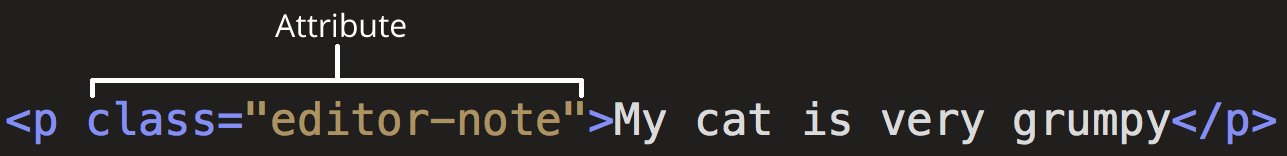
\includegraphics[width=0.7\linewidth]{figs/grumpy-cat-attribute-small} 
\end{center}
\begin{itemize}
\item
  Contain extra information about the element, but won't appear in the
  content.
\item
  Attributes such as \emph{class} and \emph{id} can be used to group
  elements. These groups can be styled in specific ways using CSS (more
  on this later).
\end{itemize}
\end{frame}

\begin{frame}[fragile]{Anatomy of a HTML Document}

\begin{columns}[T]
\begin{column}{7cm}
\begin{lstlisting}
<!DOCTYPE html>
<html lang="en-US">
  <head>
    <meta charset="utf-8" />
    <title>My test page</title>
  </head>
  <body>
    <p>This is my page</p>
  </body>
</html>
\end{lstlisting}
\end{column}

\begin{column}{7cm}
\begin{enumerate}
\item
  \texttt{DOCTYPE}: a historical artifact.
\item
  \texttt{html}: The root element. It wraps all the content on the page.
\item
  \texttt{head}: The content here does \emph{NOT} appear on the page. This is
  where styles are declared, Javascript functions are usually declared
  here too.
\item
  \texttt{title}: Appears on the browser tab. It is also what appears in the
  bookmarks page.
\item
  \texttt{body}: This contains all the content that appears on the page.
\end{enumerate}
\end{column}
\end{columns}
\end{frame}

\begin{frame}[fragile]{Running a Web-server}
\begin{itemize}
\item
  Sometimes, we may need to run a web-server on our local host to test
  the web-page properly. In such situations, we have two options:
\begin{enumerate}
\item
  Activate our python 3 virtual environment, and run
\begin{lstlisting}
python -m http.server
\end{lstlisting}

\item
  Use an nginx docker container:
\begin{lstlisting}
 docker run --name test-nginx -p8000:80 --rm \
 -v <path-to-html-pages>:/usr/share/nginx/html \
 -d nginx
\end{lstlisting}
\end{enumerate}
\item If you then navigate to \texttt{http://127.0.0.1:8000/<page-name>/}, you should 
see your web-page rendered.
\end{itemize}

\end{frame}

\subsection{CSS Basics}
\frame{\tableofcontents[currentsubsection]}

\begin{frame}{Cascading Style Sheets}
\begin{itemize}
\item
  Using HTML alone for websites would result in a very boring internet.
\item
  CSS allows us to customise how elements and layouts are presented to a
  reader.
\item
  CSS can be used to
  \begin{itemize}
  \item
    modify the font, colour, background of elements.
  \item
    change the layout, from 1-column to 3-column, for example.
  \item
    change the amount of space that an element takes up.
  \item
    include animation.
  \end{itemize}
\item
  With R and Python, quite a bit of the layout can be done without
  touching CSS directly.
\item
  However, sometimes we may want to modify things, or something may not
  be doing exactly what we wanted it to. In those situations, we may
  need to look under the hood to understand what's going on. That is our
  aim here.
\end{itemize}
\end{frame}

\begin{frame}[fragile]{CSS Syntax}
\begin{columns}[T]
\begin{column}{6cm}
\begin{lstlisting}
h1 {
  color: red;
  font-size: 5em;
}
\end{lstlisting}
\end{column}

\begin{column}{8cm}
\begin{itemize}
\item
  On the left is a single CSS rule.
\item
  The rule opens with a selector.
\item
  The curly braces contain one or more declarations.
\item
  Declarations take the form of property: value pairs, followed by a
  semi-colon.
\item
  The rule above instructs the browser to display the content of h1
  elements in red, with a particular font size.
\end{itemize}
\end{column}
\end{columns}
\end{frame}

\begin{frame}[fragile]{Adding CSS to our document}
There are three ways we can incorporate CSS into our documents.
\begin{enumerate}
\item
  Create a file (with extension css), containing all the rules, and link
  to it from within the HTML page.
\begin{lstlisting}
<link rel="stylesheet" href="styles.css" />
\end{lstlisting}
Within the css file, we can import other css files.

\item
  Include all the rules in the document header, under the
  \texttt{\textless{}style\textgreater{}} element.
\item
  Specify the style for specific elements within the style attribute.
\begin{lstlisting}
<h1 style="color: blue;background-color: red;border: 1px black;">
  Hello World!
</h1>
\end{lstlisting}
\end{enumerate}
\end{frame}

\begin{frame}[fragile]{CSS Selectors}
\begin{itemize}
\item
  The selector is the first part of a CSS rule.
\item
  It is a pattern that tells the browser which HTML elements should be
  selected to have the CSS property values inside the declaration.
\item
  Type, class and ID selectors:
\begin{lstlisting}
h1 { } 
.box { }
#unique { }
\end{lstlisting}
\item
  Combining selectors:
  \begin{itemize}
  \item
    Comma can be used to combine selectors: \texttt{A,B} means A or B
    element.
  \item
    \texttt{A.className} selects elements of type A with class
    \texttt{className}.
  \item
    \texttt{A\ B} refers to elements of type B nested within type A
    elements.
  \end{itemize}
\item
  There are numerous other rules. Try this
  \href{https://flukeout.github.io/}{excellent website} to practice with
  it.
\end{itemize}
\end{frame}

\begin{frame}{Cascade, Inheritance and Specificity Rules}
\begin{itemize}
\item
  When more than one rule applies to an element, there are several
  considerations that the browser uses to decide which one to use.
\item
  Rules that are later on in the style sheet take precedence.
\item
  Rules that are more specific take more precedence too.
\item
  It is sometimes easier to use the browser tools to understand which
  CSS rule is being applied to which element.
\end{itemize}
\end{frame}

\begin{frame}{CSS Box Model}
\begin{columns}[T]
\begin{column}{7.5cm}
Everything in CSS has a box around it. The standard box is defined by
these dimensions:
\begin{center}
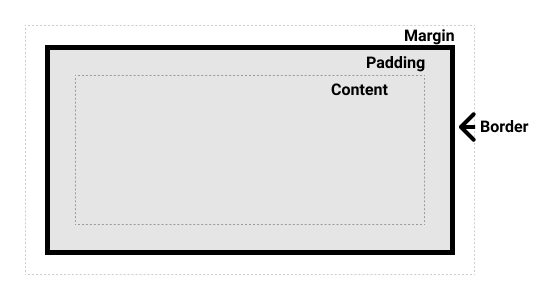
\includegraphics[width=0.7\linewidth]{figs/box-model-1.png} 
\end{center}
\end{column}
\begin{column}{7.5cm}
\begin{itemize}
\item Content: Size it using \texttt{inline-size}, \texttt{block-size}, \texttt{width} and \texttt{height}.
\item Padding: It sits around the content as white space. Size it using \texttt{padding}.
\item Border: It wraps the content and padding. Size it using \texttt{border}.
\item Margin: It serves as the space between this element and others. Size it using \texttt{margin}.
\end{itemize}
\end{column}
\end{columns}
\end{frame}

\subsection{References}

\begin{frame}{References}
\begin{enumerate}
\item
  Links from Mozilla Developer Network (MDN):
  \begin{itemize}
  \item
    \href{https://developer.mozilla.org/en-US/docs/Learn/HTML}{Introduction to HTML}
  \item
    \href{https://developer.mozilla.org/en-US/docs/Learn/CSS}{Introduction to CSS}
  \item
    \href{https://developer.mozilla.org/en-US/docs/Web/CSS/CSS_Colors/Color_picker_tool}{Colour-picker from MDN}
  \item
    \href{https://developer.mozilla.org/en-US/docs/Learn/CSS/Building_blocks/Values_and_units}{CSS values and units}
  \end{itemize}
\item
  \href{https://shiny.rstudio.com/articles/css.html}{Using CSS with Shiny}
\item
  \href{https://fonts.google.com/}{Fonts from Google}
\end{enumerate}
\end{frame}

\section{Other Interactive Components in R}
\subsection{Interactive Plots with Plotly}
\frame{\tableofcontents[currentsubsection]}

\begin{frame}[fragile]{Plotly}

\begin{itemize}
\item Plotly is an R package for creating interactive plots.
\item \texttt{ggplot} objects can easily be converted to plotly objects.

\begin{lstlisting}
library(ggplot2)
library(plotly)

# Create a ggplot object:
g1 <- qplot(x=1:3, y=2:4, col=as.factor(1:3))
# Convert it to plotly:
ggplotly(g1)
\end{lstlisting}

\item There are numerous examples that you can learn from at the 
\href{https://plotly.com/r/}{plotly R website.}

\item There is also a Python version that you can use with dash.
\end{itemize}

\end{frame}


\subsection{Interactive Dashboards from R Markdown}
\frame{\tableofcontents[currentsubsection]}

\begin{frame}{flexdashboard R package}
\begin{itemize}
\item
  Flexdashboards are dashboards that are constructed from Rmd documents.
\item It is possible to achieve column layouts, tabbed layouts just by
specifying them within the Rmd document - no need for Shiny components.
\item The difference between dashboards and Shiny is that, although dashboards
may include interactive plots and tables, they do not typically deal with user inputs like
Shiny does.
\item
  Flexdashboards \emph{can} include Shiny components, and they can also be
  served using a Shiny server, but they are meant more for automatic report
  generation and interactive visualisation of data and tables.
\item Read more about flexdashboard from their
\href{https://pkgs.rstudio.com/flexdashboard/articles/using.html}{documentation website}.
\end{itemize}
\end{frame}

\begin{frame}[fragile]{Index of Examples in Class Github Repository}
\begin{lstlisting}
- flex_eg       | Example of flexdashboard, with custom CSS
              --|--
- html_css      | Example of CSS styling HTML pages: 
                | - with div blocks
                | - modifying padding (box model)
                | - using flex layout by hand.
              --|--
- shiny_css_eg  | Example of modifying Shiny application with CSS
              --|--
- shiny_eg      | Example of containerised Shiny application
                | - installs packages on server container
                | - communicates with flask application
                | - uses docker compose
              --|--
\end{lstlisting}
\end{frame}



\end{document}
